\section{Generación de señalamiento paso a paso}

	Inicialmente, el RNA ejecuta el Algoritmo \ref{alg:graph_network} (ver Sección \ref{sec:grafos}) para detectar todos los \textit{netElements}, sus coordenadas iniciales y finales en la topología, y el sentido en el que fueron definidas. Al concluir el Algoritmo \ref{alg:graph_network}, el RNA ejecuta el Algoritmo \ref{alg:connectedness} (ver Sección \ref{sec:grafos}) para analizar la conexidad de la red. El resultado obtenido se muestra en el Código \ref{lst:EJ9_1}, donde se describen las coordenadas de cada \textit{netElement} y se confirma que la red es conexa.
	
	\begin{lstlisting}[language = {}, caption = Detección de \textit{netElements} por parte del RNA , label = {lst:EJ9_1}]
		###### Starting Railway Network Analyzer #####
		Reading .railML file
		Creating railML object
		Analysing railML object
		Analysing graph
		ne3 [9384, 0] [7584, 0] <<
		ne40 [1680, 0] [3796, 0] >>
		ne46 [3796, 0] [7584, 0] >>
		ne48 [4216, 420] [3796, 0] <<
		ne49 [4216, 420] [7164, 420] >>
		ne50 [7164, 420] [4216, 420] <<
		ne53 [7164, 420] [7584, 0] >>
		The network is connected
	\end{lstlisting}
	
	Por ejemplo, el \textit{netElement} ne50 inicia en la coordenada (7164;420) y finaliza en la coordenada (4216;420). El símbolo $<<$ indica que ne50 se encuentra definido de derecha a izquierda, ya que la componente x de la coordenada final es menor a la de la coordenada inicial, teniendo la misma componente y. Además, se puede comprobar que la lista obtenida en consistente con la Figura \ref{fig:EJ9_2}. Por ejemplo, ne48, ne49 y ne50 comparten la coordenada (4216;420), que coincide con la coordenada del cambio de vías Sw29.
	
	A continuación, el RNA detectará la infraestructura ferroviaria, las curvas peligrosas y los puntos medios de los netElements que el RNA considera demasiado largos. El análisis de la infraestructura se detalla en la Sección \ref{sec:bufferstop}, Sección \ref{sec:detectors}, Sección \ref{sec:platform} y Sección \ref{sec:crossing}, mientras que la detección de curvas y puntos medios se detalla en la Sección \ref{sec:tracks}. El RNA ejecuta el Algoritmo \ref{alg:switches_1}, Algoritmo \ref{alg:switches_2} y Algoritmo \ref{alg:switches_3} para confirmar la detección de cambios de vías simples, dobles y en tijeras. El resultado de este proceso se puede visualizar en el Código \ref{lst:EJ9_2}.
	
	\begin{lstlisting}[language = {}, caption = Detección de puntos críticos por parte del RNA , label = {lst:EJ9_2}]
		Analysing infrastructure --> Infrastructure.RNA
		Detecting Danger --> Safe_points.RNA
		ne3 has a RailJoint[J16] @ [7864, 0]
		ne3 has a RailJoint[J17] @ [8219, 0]
		ne3 has a RailJoint[J18] @ [8867, 0]
		ne3 has a Platform[Plat10] @ [8542, 0]
		ne40 has a RailJoint[J19] @ [3428, 0]
		ne40 has a RailJoint[J20] @ [2485, 0]
		ne40 has a RailJoint[J21] @ [2149, 0]
		ne40 has a Platform[Plat14] @ [2848, 0]
		ne46 has a RailJoint[J12] @ [4952, 0]
		ne46 has a RailJoint[J15] @ [6424, 0]
		ne46 has a Platform[Plat13] @ [5487, 0]
		ne46 has a LevelCrossing[Lc10] @ [5915, 0]
		ne49 has a RailJoint[J10] @ [4952, 870]
		ne49 has a RailJoint[J13] @ [6424, 870]
		ne49 has a Platform[Plat11] @ [5487, -870]
		ne49 has a LevelCrossing[Lc11] @ [6006, -870]
		ne49 has a Curve(3 lines) @ [[4666, 870], [6714, 870]]
		ne50 has a RailJoint[J11] @ [4952, 420]
		ne50 has a RailJoint[J14] @ [6424, 420]
		ne50 has a Platform[Plat12] @ [5487, -420]
		ne50 has a LevelCrossing[Lc09] @ [6096, -420]
	\end{lstlisting}
	
	Esta información es exportada por el RNA, con mayor detalle, en el archivo Infrastructure.RNA (Código \ref{lst:EJ9_4}) que resume cada elemento ferroviario asociado a su respectivo \textit{netElement}.

	\begin{lstlisting}[language = {}, caption = Infrastructure.RNA, label = {lst:EJ9_4}]
Nodes: 7|Switches: 4|Signals: 0|Detectors: 12|Ends: 2|Barriers: 3
Node ne3:
	Track = track2
	TrainDetectionElements -> tde83
		Type -> insulatedRailJoint
	TrainDetectionElements -> tde84
		Type -> insulatedRailJoint
	TrainDetectionElements -> tde85
		Type -> insulatedRailJoint
	Type = BufferStop -> ['bus5']
	Neighbours = 2 -> ['ne46', 'ne53']
	Switches -> Sw31
		ContinueCourse -> left -> ne46
		BranchCourse -> right -> ne53
Node ne40:
	Track = track1
	TrainDetectionElements -> tde86
		Type -> insulatedRailJoint
	TrainDetectionElements -> tde87
		Type -> insulatedRailJoint
	TrainDetectionElements -> tde88
		Type -> insulatedRailJoint
	Type = BufferStop -> ['bus1']
	Neighbours = 2 -> ['ne46', 'ne48']
	Switches -> Sw27
		ContinueCourse -> right -> ne46
		BranchCourse -> left -> ne48
Node ne46:
	Track = track3
	TrainDetectionElements -> tde71
		Type -> insulatedRailJoint
	TrainDetectionElements -> tde82
		Type -> insulatedRailJoint
	Neighbours = 4 -> ['ne3', 'ne40', 'ne48', 'ne53']
	Level crossing -> Lc10
		Protection -> true | Barriers -> none | Lights -> none Acoustic -> none
		Position -> [5960, 0] | Coordinate: 0.5712
Node ne48:
	Track = track4
	Neighbours = 4 -> ['ne40', 'ne46', 'ne49', 'ne50']
	Switches -> Sw29
		ContinueCourse -> left -> ne49
		BranchCourse -> right -> ne50
Node ne49:
	Track = track5
	TrainDetectionElements -> tde69
		Type -> insulatedRailJoint
	TrainDetectionElements -> tde80
		Type -> insulatedRailJoint
	Neighbours = 3 -> ['ne48', 'ne50', 'ne53']
	Level crossing -> Lc11
		Protection -> true | Barriers -> none | Lights -> none Acoustic -> none
		Position -> [6051, -870] | Coordinate: 0.6086
Node ne50:
	Track = track6
	TrainDetectionElements -> tde70
		Type -> insulatedRailJoint
	TrainDetectionElements -> tde81
		Type -> insulatedRailJoint
	Neighbours = 3 -> ['ne48', 'ne49', 'ne53']
	Level crossing -> Lc09
		Protection -> true | Barriers -> none | Lights -> none Acoustic -> none
		Position -> [6051, -420] | Coordinate: 0.3776
Node ne53:
	Track = track7
	Neighbours = 4 -> ['ne3', 'ne46', 'ne49', 'ne50']
	Switches -> Sw33
		ContinueCourse -> right -> ne49
		BranchCourse -> left -> ne50
	\end{lstlisting}

	La información de la infraestructura es utilizada por el RNA para detectar los puntos críticos de la red, es decir, las zonas donde es recomendable colocar una señal, según el sentido de circulación que se desee. El resultado es exportado al archivo SafePoints.RNA (Código \ref{lst:EJ9_5}). En el caso de que un mismo \textit{netElement} tenga más de un punto crítico para el mismo sentido, el RNA tomará el más cercano al elemento a proteger. El criterio de selección de puntos críticos se aplica para cada elemento ferroviario detectado, cada curva y cada cambio de vías y fue explicado en las secciones correspondientes ya mencionadas.

	\begin{lstlisting}[language = {}, caption = SafePoints.RNA, label = {lst:EJ9_5}]
ne3:
	Next: [[7764.0, 0], [8119.0, 0], [8767.0, 0]]
	Prev: [[7964.0, 0], [8319.0, 0], [8967.0, 0]]
ne40:
	Next: [[3328.0, 0], [2385.0, 0], [2049.0, 0]]
	Prev: [[3528.0, 0], [2585.0, 0], [2249.0, 0]]
ne46:
	Next: [[4852.0, 0], [6324.0, 0], [5715, 0]]
	Prev: [[5052.0, 0], [6524.0, 0], [6115, 0]]
ne49:
	Next: [[4852.0, 870], [6324.0, 870], [5806, -870], [6614.0, 870]]
	Prev: [[5052.0, 870], [6524.0, 870], [6206, -870], [4766.0, 870]]
ne50:
	Next: [[4852.0, 420], [6324.0, 420], [5896, -420]]
	Prev: [[5052.0, 420], [6524.0, 420], [6296, -420]]
	\end{lstlisting}	
	
	Una vez que el RNA detectó cada punto crítico de la red ferroviaria, procede a generar el señalamiento. El orden en que se procesan los elementos ferroviarios no impacta en el resultado final, pero para poder describirlo de forma ordenada se iniciará generando el señalamiento para proteger los finales de vías, las junturas entre rieles, las plataformas (explicado en la Sección \ref{sec:sig_platform}), los cruces de vía (explicado en la Sección \ref{sec:sig_levelcrossing}) y los cambios de vías (explicado en la Sección \ref{sec:signal_switches}). Luego se procederá a mostrar el señalamiento completo antes y después de la simplificación de señales (explicado en la Sección \label{sec:simplificacion}). 
	
	Tal cómo se explicó en la Sección \ref{sec:sig_border}, el RNA aplica el Algoritmo \ref{alg:lineBorder} y el Algoritmo \ref{alg:bufferStop} para generar las señales para proteger los finales de vías relativos y absolutos. Estas señales son ilustradas en la Figura \ref{fig:EJ9_3}.

	\begin{figure}[H]
		\centering
		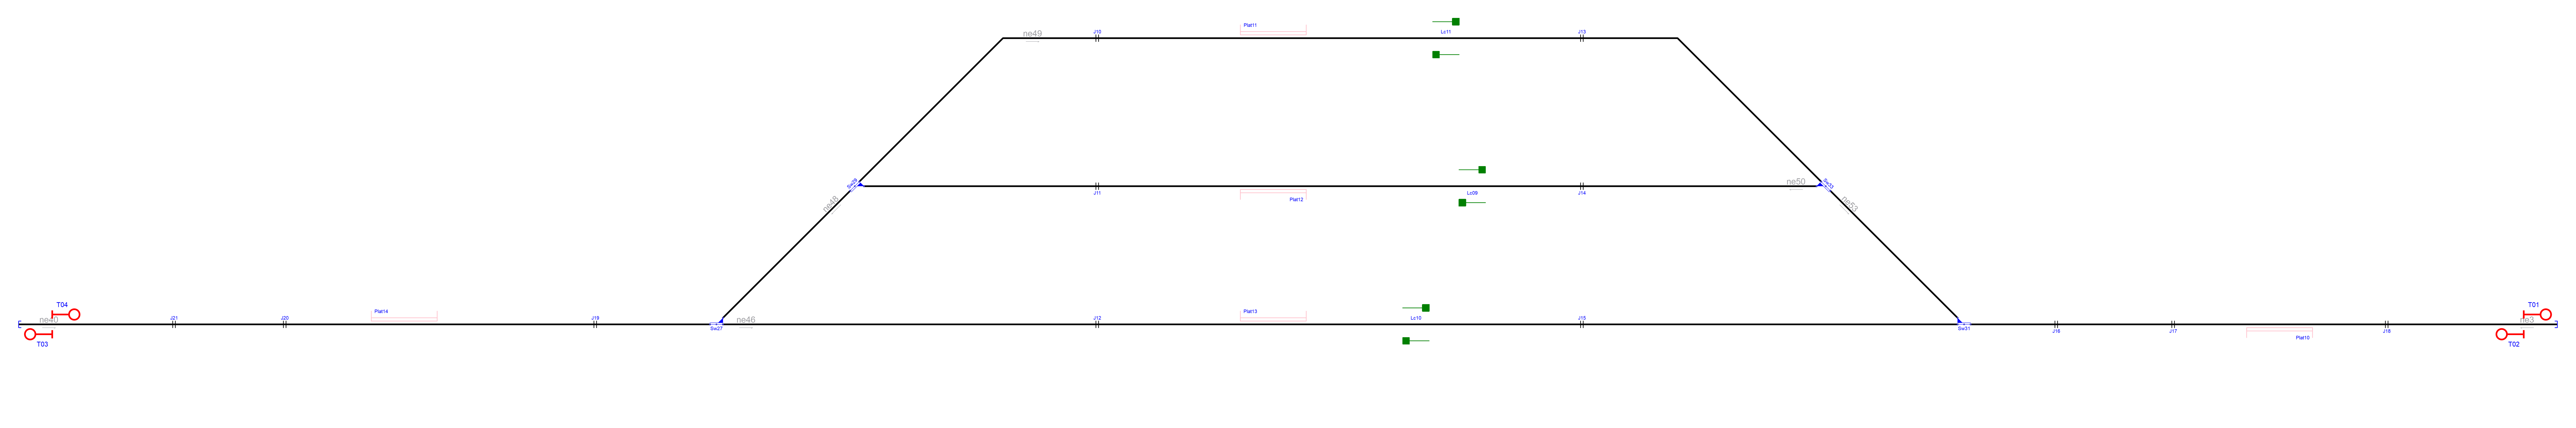
\includegraphics[width=1\textwidth]{resultados-obtenidos/ejemplo9/images/9_step1.png}
		\centering\caption{Señalamiento generado por el RNA para proteger el fin de vía.}
		\label{fig:EJ9_3}
	\end{figure}

	Los finales de vías absolutos son protegidos por las señales de parada T01 y T03, y las señales de partida son T02 y T04. A su vez, al no existir los finales de vías relativos, el RNA no les asignó ninguna señal para su protección.

	La Figura \ref{fig:EJ9_4} ilustra la generación de señales destinadas a proteger las junturas entre los rieles. Estas señales se obtuvieron al aplicar el Algoritmo \ref{alg:RJ}, tal como fue explicado en la Sección \ref{sec:sig_joint} Las señales generadas son todas las señales entre J05 y J28, indicadas en color rojo.

	\begin{figure}[H]
		\centering
		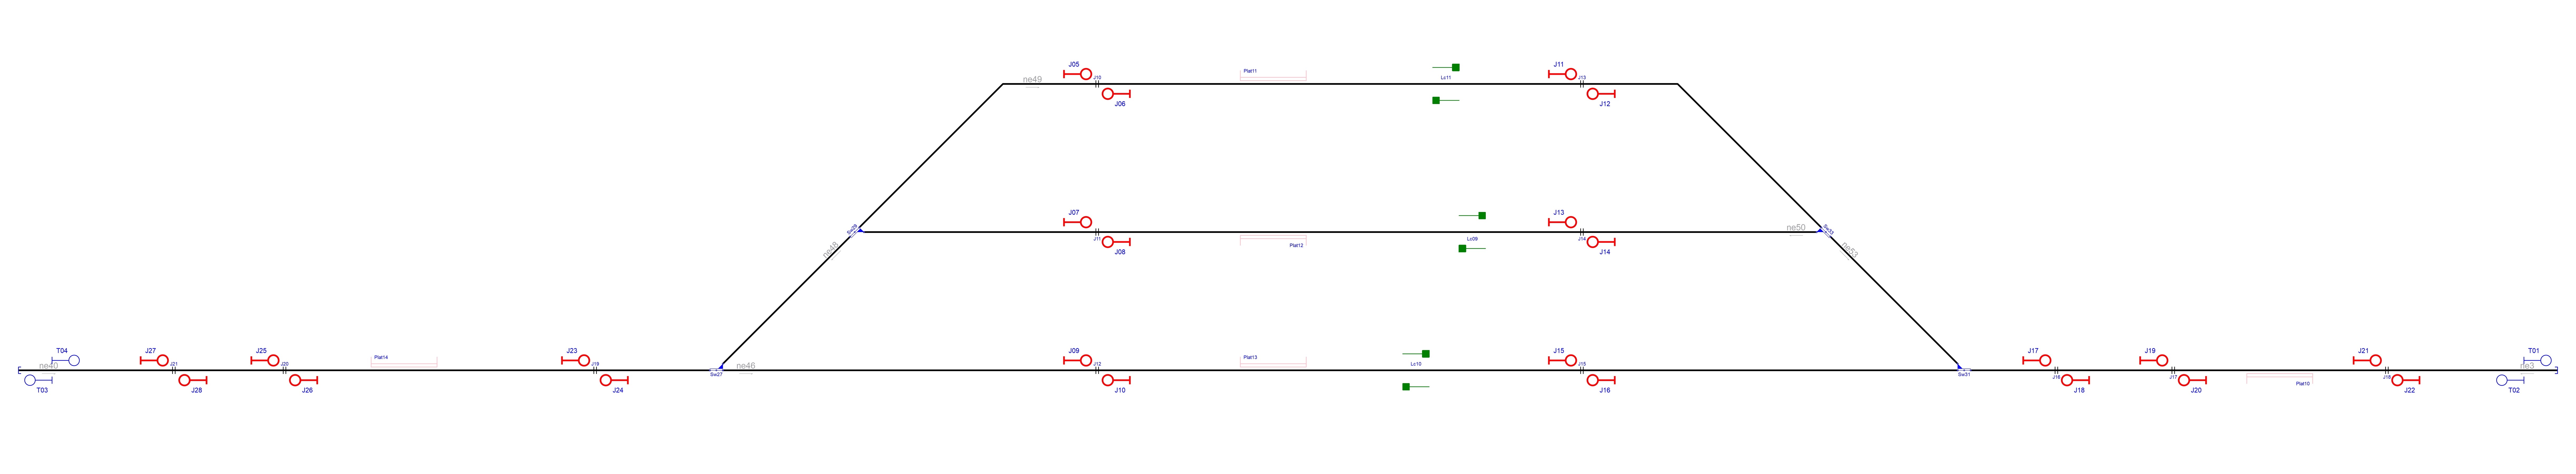
\includegraphics[width=1\textwidth]{resultados-obtenidos/ejemplo9/images/9_step2.png}
		\centering\caption{Señalamiento generado por el RNA para proteger las junturas.}
		\label{fig:EJ9_4}
	\end{figure}

	Al generar el señalamiento para proteger la infraestructura, tal como se explicó en la Sección \ref{sec:horizontal}, el Algoritmo \ref{alg:horizontal} simplificará las señales entre dos elementos ferroviarios si no existe espacio suficiente entre ellos, tal como sucede con los elementos LevelCrossing09 y Platorm12. El señalamiento generado para proteger las plataformas y los cruces de vía se ilustra en rojo en la Figura \ref{fig:EJ9_5}. Las señales generadas para proteger las plataformas no fueron generadas, al encontrarse próximas a las señales de protección de junturas, por lo que el RNA decidió no superponer ambas señales. Mientras que las señales que protegen los cruces de vía son las señales X29 a X34.

	\begin{figure}[H]
		\centering
		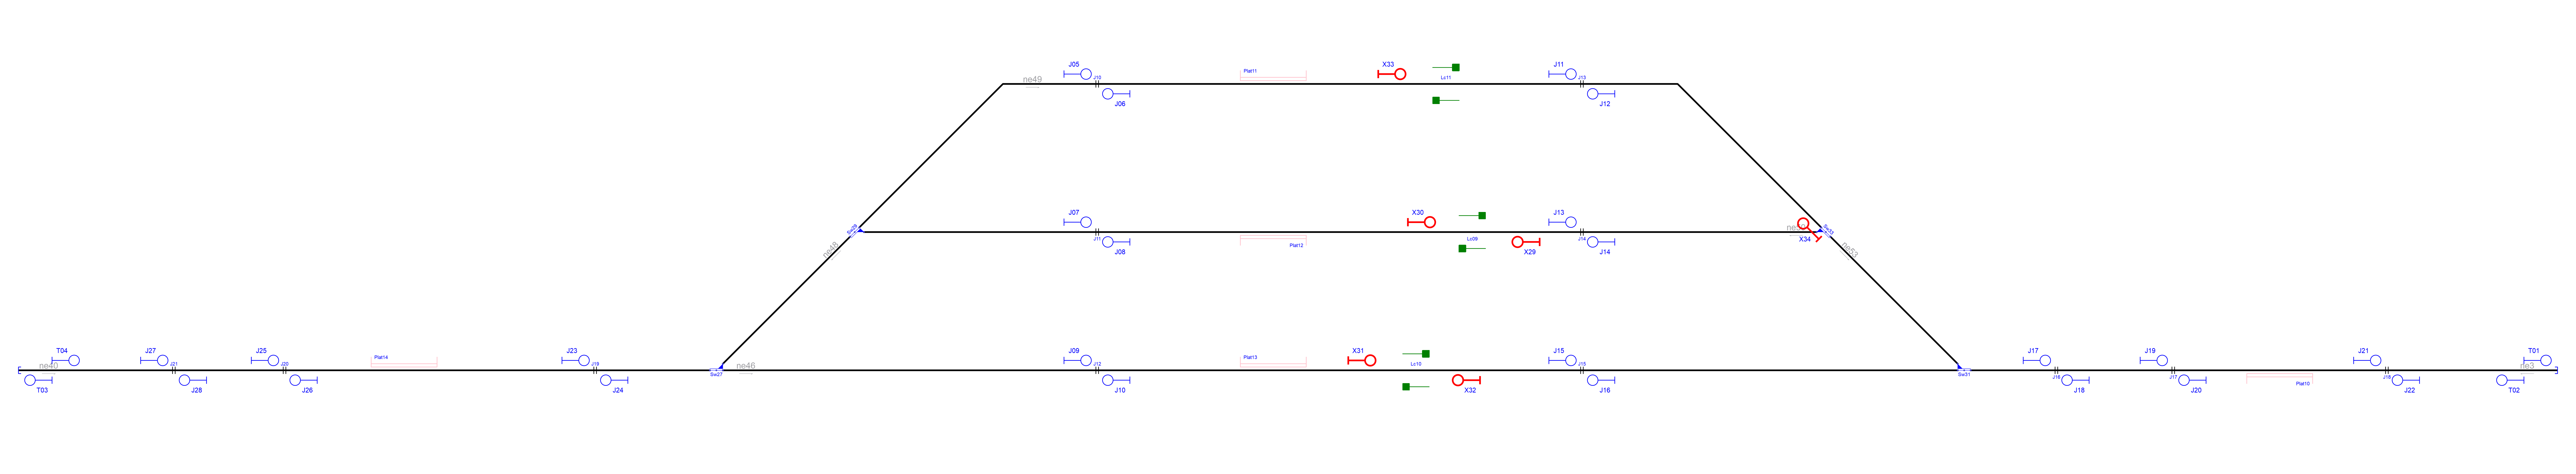
\includegraphics[width=1\textwidth]{resultados-obtenidos/ejemplo9/images/9_step3.png}
		\centering\caption{Señalamiento generado por el RNA para proteger plataformas y cruces de vía.}
		\label{fig:EJ9_5}
	\end{figure}

	Al aplicar el Algoritmo \ref{alg:SW} de generación de señalamiento para cambios de vías, tal como fue explicado en la Sección \label{sec:signal_switches}, el RNA genera  las señales S36 , C35, H36 y H38 para proteger el cambio de vías Sw27; las señales S42, C41, H43 y H44 para proteger el cambio de vías Sw31; las señales C39 y B46 para proteger el cambio de vías Sw29 y la señal C45 para proteger el cambio de vías Sw33. Las señales mencionadas se encuentran resaltadas en rojo en la Figura \ref{fig:EJ9_6}.

	\begin{figure}[H]
		\centering
		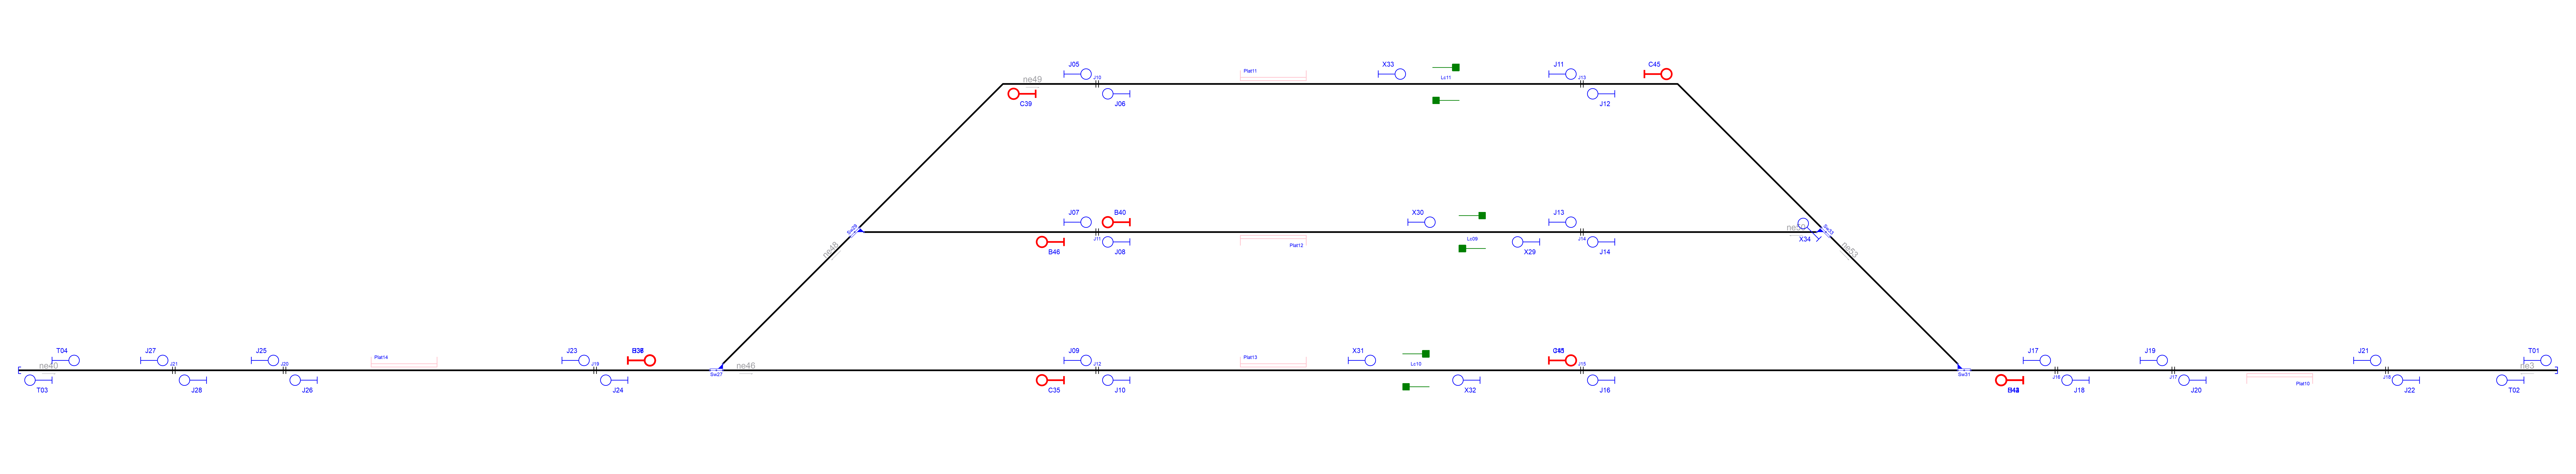
\includegraphics[width=1\textwidth]{resultados-obtenidos/ejemplo9/images/9_step4.png}
		\centering\caption{Señalamiento generado por el RNA para proteger los cambios de vías.}
		\label{fig:EJ9_6}
	\end{figure}

	Una vez obtenido todo el señalamiento, el RNA procede a simplificar las señales redundantes, repetidas o cuyas funciones o ubicaciones se superponen entre sí. El proceso de simplificación de señales fue explicado en la Sección \ref{sec:simplificacion}. El Algoritmo \ref{alg:vertical} de herencia vertical fue aplicado en las señales B entre los cambios de vías Sw31 y Sw33, desplazando las señales hasta convertirlas en las señales H43 y H respectivamente. Análogamente, entre los cambios de vías Sw27 y Sw29 se convirtieron en las señales H37 y H38 respectivamente.
	
	Las señales simplificadas al aplicar el Algoritmo \ref{alg:horizontal} de herencia horizontal son: J22, J28, J27, C39, J08, C35, C45, X34, X30, X29, J15, X32, J19, J20, J18, J23, H37, H38, B40, H43 y H44. Las señales J23, H37 y H38 fueron eliminadas por su cercanía con la señal S36, con la cual comparten dirección y sentido. Lo mismo ocurre entre el par de señales H43/H44 y la señal S42; además de varios otros casos de simplificaciones simples. En todos los casos, se aplicó el Algoritmo \ref{alg:horizontal}, diseñado para agrupar objetos cercanos como un único objeto, generando el señalamiento acorde a los elementos contenidos en cada extremo del nuevo elemento contenedor.
	
	Finalmente, las señales son simplificadas aplicando el Algoritmo \ref{alg:reduction} de eliminación por prioridad de señales. El resultado de este proceso es detallado en el Código \ref{lst:EJ9_3}.

	\begin{lstlisting}[language = {}, caption = Reducción de señalamiento por prioridad de señales, label = {lst:EJ9_3}]
Reducing redundant signals
removing J22 for T02
removing J28 for T03
removing J27 for T04
removing C39 for J06
removing J08 for B40
removing C35 for J10
removing C45 for J11
removing X34 for J12
removing X30 for J13
removing X29 for J14
removing J15 for C41
removing X32 for J16
removing J19 for J17
removing J20 for J18
removing J18 for S42
removing J23 for S36
removing H37 for S36
removing H38 for S36
removing B40 for B46
removing H43 for S42
removing H44 for S42
	\end{lstlisting}

	El resultado de la simplificación del señalamiento se ilustra en la Figura \ref{fig:EJ9_7}.
	
	\begin{figure}[H]
		\centering
		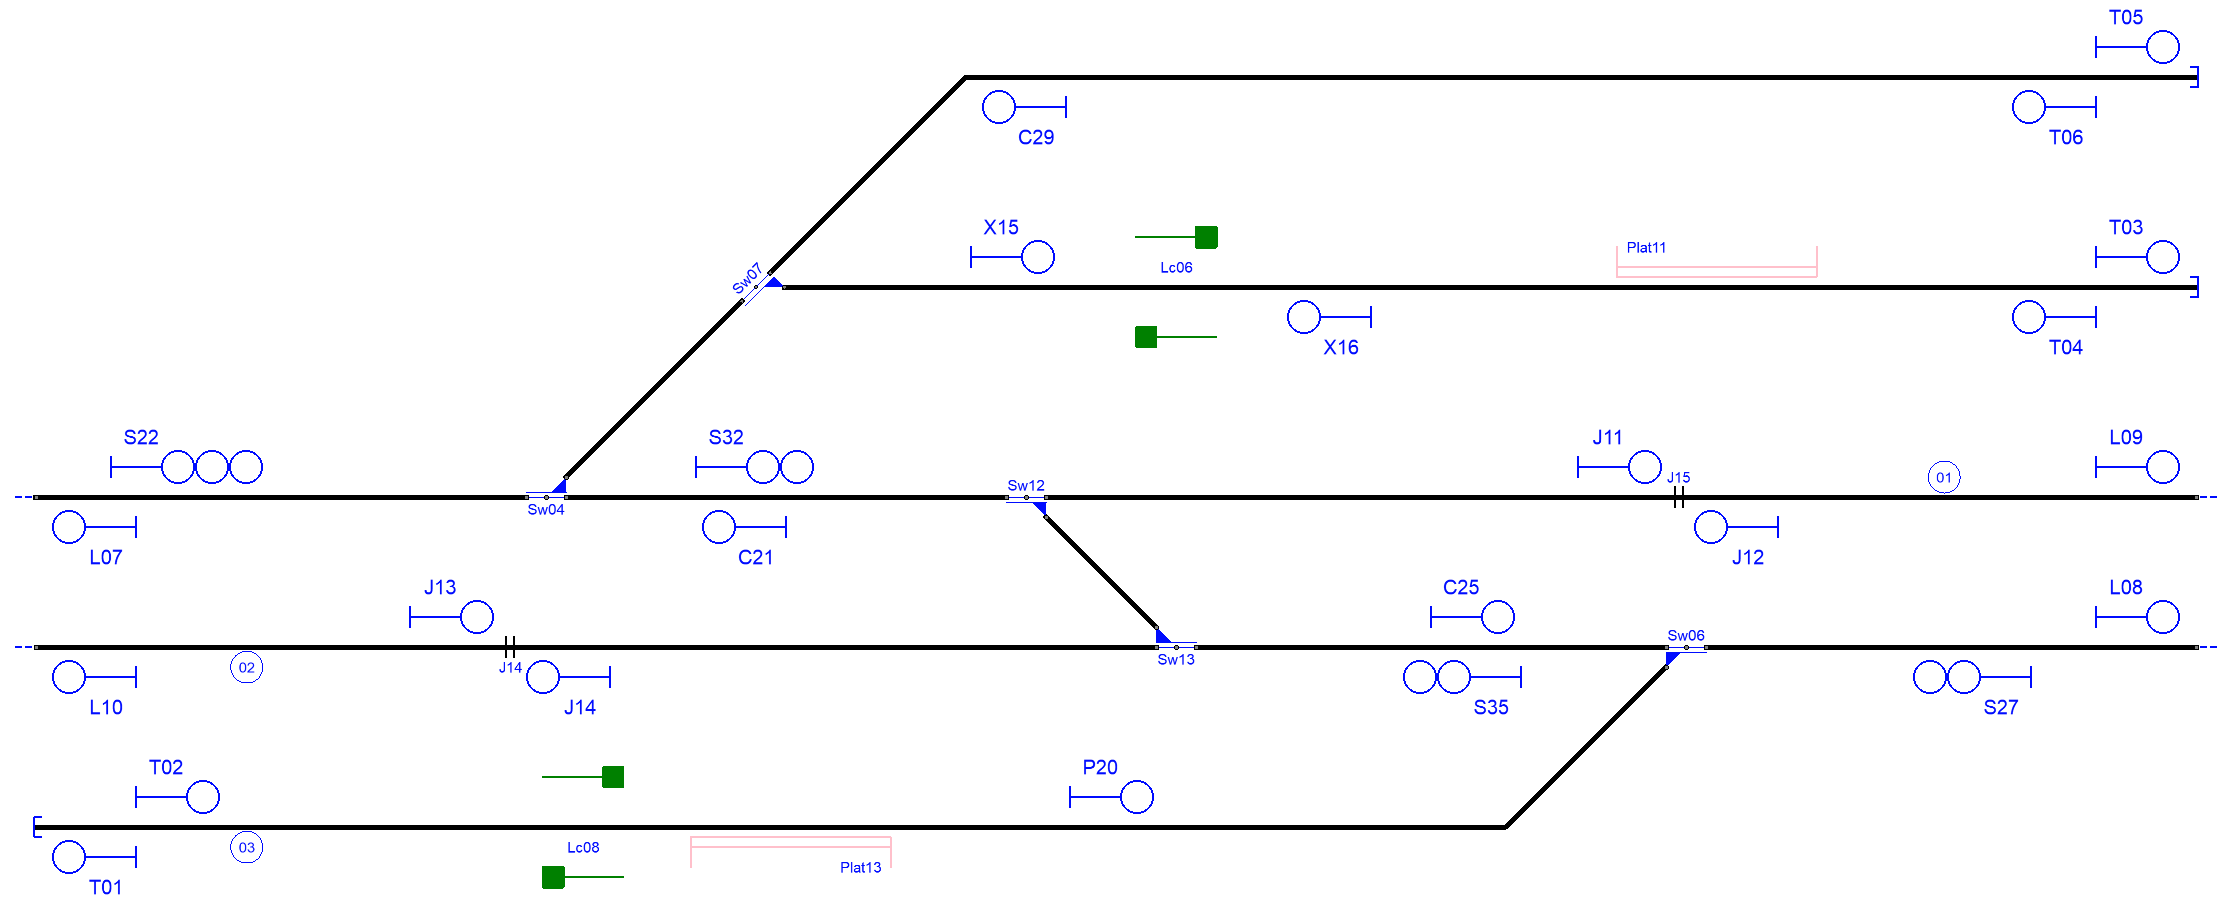
\includegraphics[width=1\textwidth]{resultados-obtenidos/ejemplo1/images/1_RNA.png}
		\centering\caption{Señalamiento generado y simplificado por el RNA.}
		\label{fig:EJ9_7}
	\end{figure}
	
	Además, toda la información del señalamiento generado es exportada por el RNA en el archivo Signalling.RNA (Código \ref{lst:EJ1_6}), que incluye información detallada de la posición, orientación, sentido, coordenada, nombre y tipo de señal.
	
	\begin{lstlisting}[language = {}, caption = Signalling.RNA, label = {lst:EJ9_6}]
T01 [T01] >>:
	From: ne3 | To: bus5_right
	Type: Stop | Direction: reverse | AtTrack: right 
	Position: [9284, 0] | Coordinate: 0.9444
T02 [T02] <<:
	From: ne3 | To: ne3_left
	Type: Stop | Direction: normal | AtTrack: left 
	Position: [9284, 0] | Coordinate: 0.9444
T03 [T03] <<:
	From: ne40 | To: bus1_left
	Type: Stop | Direction: reverse | AtTrack: right 
	Position: [1780, 0] | Coordinate: 0.0472
T04 [T04] >>:
	From: ne40 | To: ne40_right
	Type: Stop | Direction: normal | AtTrack: left 
	Position: [1780, 0] | Coordinate: 0.0472
J05 [J05] >>:
	From: ne49 | To: ne49_right
	Type: Circulation | Direction: normal | AtTrack: left 
	Position: [4852.0, -870] | Coordinate: 0.4392
J06 [J06] <<:
	From: ne49 | To: ne49_left
	Type: Circulation | Direction: reverse | AtTrack: right 
	Position: [5052.0, -870] | Coordinate: 0.4995
J07 [J07] >>:
	From: ne50 | To: ne50_right
	Type: Circulation | Direction: reverse | AtTrack: right 
	Position: [4852.0, -420] | Coordinate: 0.2157
J09 [J09] >>:
	From: ne46 | To: ne46_right
	Type: Circulation | Direction: normal | AtTrack: left 
	Position: [4852.0, 0] | Coordinate: 0.2787
J10 [J10] <<:
	From: ne46 | To: ne46_left
	Type: Circulation | Direction: reverse | AtTrack: right 
	Position: [5052.0, 0] | Coordinate: 0.3315
J11 [J11] >>:
	From: ne49 | To: ne49_right
	Type: Circulation | Direction: normal | AtTrack: left 
	Position: [6324.0, -870] | Coordinate: 0.8825
J12 [J12] <<:
	From: ne49 | To: ne49_left
	Type: Circulation | Direction: reverse | AtTrack: right 
	Position: [6524.0, -870] | Coordinate: 0.9427
J13 [J13] >>:
	From: ne50 | To: ne50_right
	Type: Circulation | Direction: reverse | AtTrack: right 
	Position: [6324.0, -420] | Coordinate: 0.7150
J14 [J14] <<:
	From: ne50 | To: ne50_left
	Type: Circulation | Direction: normal | AtTrack: left 
	Position: [6524.0, -420] | Coordinate: 0.7829
J16 [J16] <<:
	From: ne46 | To: ne46_left
	Type: Circulation | Direction: reverse | AtTrack: right 
	Position: [6524.0, 0] | Coordinate: 0.7201
J17 [J17] >>:
	From: ne3 | To: ne3_right
	Type: Circulation | Direction: reverse | AtTrack: right 
	Position: [7764.0, 0] | Coordinate: 0.1
J21 [J21] >>:
	From: ne3 | To: ne3_right
	Type: Circulation | Direction: reverse | AtTrack: right 
	Position: [8767.0, 0] | Coordinate: 0.6572
J24 [J24] <<:
	From: ne40 | To: ne40_left
	Type: Circulation | Direction: reverse | AtTrack: right 
	Position: [3528.0, 0] | Coordinate: 0.8733
J25 [J25] >>:
	From: ne40 | To: ne40_right
	Type: Circulation | Direction: normal | AtTrack: left 
	Position: [2385.0, 0] | Coordinate: 0.3331
J26 [J26] <<:
	From: ne40 | To: ne40_left
	Type: Circulation | Direction: reverse | AtTrack: right 
	Position: [2585.0, 0] | Coordinate: 0.4276
X31 [X31] >>:
	From: ne46 | To: ne46_right
	Type: Circulation | Direction: normal | AtTrack: left 
	Position: [5715, 0] | Coordinate: 0.5065
X33 [X33] >>:
	From: ne49 | To: ne49_right
	Type: Circulation | Direction: normal | AtTrack: left 
	Position: [5806, 870] | Coordinate: 1.0096
S36 [S36] >>:
	From: ne40 | To: ne40_right
	Type: Circulation | Direction: normal | AtTrack: left 
	Position: [3528.0, 0] | Coordinate: 0.8733
C41 [C41] >>:
	From: ne46 | To: ne46_right
	Type: Circulation | Direction: normal | AtTrack: left 
	Position: [6324.0, 0] | Coordinate: 0.6673
S42 [S42] <<:
	From: ne3 | To: ne3_left
	Type: Circulation | Direction: normal | AtTrack: left 
	Position: [7764.0, 0] | Coordinate: 0.1
B46 [B46] <<:
	From: ne50 | To: ne50_right
	Type: Manouver | Direction: normal | AtTrack: left 
	Position: [4852.0, -420] | Coordinate: 0.2157
	\end{lstlisting}
	
	Al finalizar la generación del señalamiento, el RNA ejecuta el Algoritmo \ref{alg:routes}, explicado en la Sección \ref{sec:rutas}, para detectar todas las posibles rutas admitidas por la red para crear la tabla de enclavamientos. La cuál puede ser visualizada en el archivo Routes.RNA (Código \ref{lst:EJ9_7}). La misma detalla las señales de inicio y final, los \textit{netElements} abarcados por la ruta y cualquier infraestructura involucrada, incluyendo el estado que deben tener para que la ruta sea activada.
	
	\begin{lstlisting}[language = {}, caption = Routes.RNA, label = {lst:EJ9_7}]
route_1 [T02 << S42]:
	Path: ['ne3']
	Platforms: ['Plat10']
route_2 [T04 >> J25]:
	Path: ['ne40']
route_3 [J05 >> J11]:
	Path: ['ne49']
	Platforms: ['Plat11']
	LevelCrossings: ['Lc11']
route_4 [J06 << J24]:
	Path: ['ne49', 'ne48', 'ne40']
	Switches: ['Sw27_R', 'Sw29_N']
route_5 [J07 >> J13]:
	Path: ['ne50']
	Platforms: ['Plat12']
	LevelCrossings: ['Lc09']
route_6 [J09 >> X31]:
	Path: ['ne46']
	Platforms: ['Plat13']
route_7 [J10 << J24]:
	Path: ['ne46', 'ne40']
	Switches: ['Sw27_N']
route_8 [J11 >> J17]:
	Path: ['ne49', 'ne53', 'ne3']
	Switches: ['Sw31_R', 'Sw33_N']
route_9 [J12 << J06]:
	Path: ['ne49']
	Platforms: ['Plat11']
	LevelCrossings: ['Lc11']
route_10 [J13 >> J17]:
	Path: ['ne50', 'ne53', 'ne3']
	Switches: ['Sw31_R', 'Sw33_R']
route_11 [J14 << B46]:
	Path: ['ne50']
	Platforms: ['Plat12']
	LevelCrossings: ['Lc09']
route_12 [J16 << J10]:
	Path: ['ne46']
	Platforms: ['Plat13']
	LevelCrossings: ['Lc10']
route_13 [J17 >> J21]:
	Path: ['ne3']
	Platforms: ['Plat10']
route_14 [J21 >> T01]:
	Path: ['ne3']
route_15 [J24 << J26]:
	Path: ['ne40']
	Platforms: ['Plat14']
route_16 [J25 >> S36]:
	Path: ['ne40']
	Platforms: ['Plat14']
route_17 [J26 << T03]:
	Path: ['ne40']
route_18 [X31 >> C41]:
	Path: ['ne46']
	LevelCrossings: ['Lc10']
route_19 [X33 >> J17]:
	Path: ['ne49', 'ne53', 'ne3']
	Switches: ['Sw31_R', 'Sw33_N']
	LevelCrossings: ['Lc11']
route_20 [S36 >> J09]:
	Path: ['ne40', 'ne46']
	Switches: ['Sw27_N']
route_21 [S36 >> J05]:
	Path: ['ne40', 'ne48', 'ne49']
	Switches: ['Sw27_R', 'Sw29_N']
route_22 [S36 >> J07]:
	Path: ['ne40', 'ne48', 'ne50']
	Switches: ['Sw27_R', 'Sw29_R']
route_23 [C41 >> J17]:
	Path: ['ne46', 'ne3']
	Switches: ['Sw31_N']
route_24 [S42 << J16]:
	Path: ['ne3', 'ne46']
	Switches: ['Sw31_N']
route_25 [S42 << J12]:
	Path: ['ne3', 'ne53', 'ne49']
	Switches: ['Sw31_R', 'Sw33_N']
route_26 [S42 << J14]:
	Path: ['ne3', 'ne53', 'ne50']
	Switches: ['Sw31_R', 'Sw33_R']
route_27 [B46 << J24]:
	Path: ['ne50', 'ne48', 'ne40']
	Switches: ['Sw27_R', 'Sw29_R']
	\end{lstlisting}	
	
	